 The given lines  can be written as
\begin{align}
\vec{x} &= \myvec{-1\\-1\\-1} + \kappa_1\myvec{7\\-6\\1}\\
\vec{x} &= \myvec{3\\5\\7} + \kappa_2\myvec{1\\-2\\1} \\
\vec{A} = \myvec{-1\\-1\\-1},\, \vec{B} &= \myvec{3\\5\\7}, \,\vec{m}_1 = \myvec{7\\-6\\1}, \, \vec{m}_2 = \myvec{1\\-2\\1}
\end{align}
%
We first check whether the given lines are skew. The lines 
\begin{align}
\vec{x} = \vec{x_1} + \kappa_1\vec{m_1},\, \vec{x} = \vec{x_2} + \kappa_2\vec{m_2} 
\label{eq:chapters/12/11/2/15/1}
\end{align}
intersect if
\begin{align}
\vec{M}{\kappa} &= \vec{x_2} - \vec{x_1}\\
\vec{M} &\triangleq \myvec{\vec{m_1} & \vec{m_2}} \\
\bm{\kappa} &\triangleq \myvec{\kappa_1\\-\kappa_2}\\
\end{align}
Here we have,
\begin{align}
\vec{M} = \myvec{7&1\\-6&-2\\1&1}\,
\vec{x_2} - \vec{x_1} = \myvec{4\\6\\8}
\end{align}
We check whether the equation \eqref{eq:chapters/12/11/2/15/2} has a solution
\begin{align}
\myvec{7&1\\-6&-2\\1&1}\bm{\kappa} = \myvec{4\\6\\8}
\label{eq:chapters/12/11/2/15/2}
\end{align}
the augmented matrix is given by,
\begin{align}
\myvec{7&1&\vrule&4\\-6&-2&\vrule&6\\1&1&\vrule&8}
\xleftrightarrow[R_3 \leftarrow R_3 - \frac{1}{7}R_1]{R_2 \leftarrow R_2 + \frac{6}{7}R_1}\\
\myvec{7&1&\vrule&4\\&&\vrule\\0&-\frac{8}{7}&\vrule&\frac{66}{7}\\&&\vrule\\0&\frac{6}{7}&\vrule&-\frac{52}{7}}
\xleftrightarrow{R_3 \leftarrow R_3 + \frac{3}{4}R_2}\\
\myvec{2&3&\vrule&1\\&&\vrule\\0&-\frac{7}{2}&\vrule&\frac{1}{2}\\&&\vrule\\0&0&\vrule&-\frac{5}{14}}
\end{align}
The rank of the matrix is 3. So the given lines are skew.
The closest points on two skew lines defined by \eqref{eq:chapters/12/11/2/15/1} are given by 
\begin{align}
\vec{M}^\top \vec{M}\bm{\kappa} &= \vec{M}^\top\brak{\vec{x_2}-\vec{x_1}}\\
\implies \myvec{7&-6&1\\1&-2&1} \myvec{7&1\\-6&-2\\1&1}\bm{\kappa} &= \myvec{7&-6&1\\1&-2&1} \myvec{4\\6\\8}\\
\implies \myvec{86&20\\20&6}\bm{\kappa} &= \myvec{0\\0}
\label{eq:chapters/12/11/2/15/3}
\end{align}
The augmented matrix of the above equation \eqref{eq:chapters/12/11/2/15/3} is given by,
\begin{align}
\myvec{86&20&\vrule&0\\20&6&\vrule&0}
\xleftrightarrow{R_2 \leftarrow R_2 - \frac{10}{43}R_1}
\myvec{86&20&\vrule&0 \\&&\vrule\\ 0&\frac{58}{43}&\vrule&0}
\xleftrightarrow[R_2 \leftarrow \frac{43}{58}R_2]{R_1 \leftarrow \frac{1}{86} \brak{R_1 - \frac{430}{29}R_2}}\\
\myvec{1&0&\vrule&0 \\&&\vrule\\ 0&1&\vrule&0}
\end{align}
yielding
\begin{align}
\myvec{\kappa_1\\-\kappa_2} &= \myvec{0\\0}
\end{align}
The closest points $\vec{A}$ on line $l_1$ and $\vec{B}$ on line $l_2$ are given by,
\begin{align}
\vec{A} &= \vec{x_1} + \kappa_1\vec{m_1}
= \myvec{-1\\-1\\-1}\\
\vec{B} &= \vec{x_2} + \kappa_2\vec{m_2}
= \myvec{3\\5\\7}
\end{align}
The minimum distance between the lines is given by
\begin{align}
\norm{\vec{B}-\vec{A}} &= \norm{\myvec{4\\6\\8}}
= 2\sqrt{29}
\end{align}
%
\begin{figure}[!ht]
\centering
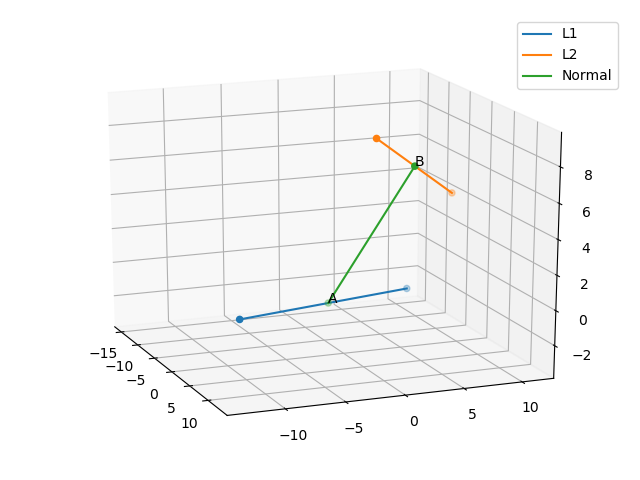
\includegraphics[width=\columnwidth]{chapters/12/11/2/15/figs/Figure_1.png}
\caption{}
\label{fig:chapters/12/11/2/15/}
\end{figure}

